\documentclass[10pt]{article}
\usepackage[margin=1.0in]{geometry} % Please keep the margins at 1.5 so that there is space for grader comments.
\usepackage{amsmath,amsthm,amssymb,tikz}
\def\mathLarge#1{\mbox{\LARGE $#1$}}

\newcommand{\overbar}[1]{\mkern 1.5mu\overline{\mkern-1.5mu#1\mkern-1.5mu}\mkern 1.5mu}

\begin{document}
\begin{center}\Large Math 492 Quantum Physics Problem\end{center}
\begin{center}\large Ryan Toepfer and Carter Ronald\end{center}

\section{Problem Statement}
We have set out to analyze how the parameters of quantam systems govern how the state of the system changes over time.

\section{Axioms and Definitions}

Definition 2.1) A complex $A$ matrix is \textbf{skew hermitian} iff its transpose conjugate is equal to $-A$.
Therefore, all $2\times2$ skew hermitian matricies fit the form
\begin{center}
$\begin{pmatrix}ai&b+ci\\-b+ci&di\end{pmatrix}$
or alternatively, 
$\begin{pmatrix}ai&\beta\\-\bar\beta&di\end{pmatrix}$
\end{center}

Axiom 2.2) The state of a quantum system can be described entirely by $\begin{pmatrix}x\\y\end{pmatrix}$, where $x,y$ are complex numbers. 

Axiom 2.3) Two quantum states are considered the same if one is a multiple of another, i.e. $\begin{pmatrix}x\\y\end{pmatrix}=\alpha\begin{pmatrix}v\\w\end{pmatrix}$ for any $x,y,\alpha,v,w\in\mathbb C$, means both states are the same.
Therefore any state $\begin{pmatrix}x\\y\end{pmatrix}$ can be represented as a ratio $z=x/y$.

Axiom 2.4) The function describing the state of a quantum system at time $t$ is the solution to the ODE
\begin{center}$
\dot{\begin{pmatrix}x\\y\end{pmatrix}}=A\begin{pmatrix}x\\y\end{pmatrix}
$\end{center}
where $A$ is a skew hermitian matrix.

\section{Initial Results}
Combining Axiom 2.4 with the general form of a $2\times2$ skew hermitian matrix gives
\begin{center}
$\dot{\begin{pmatrix}x\\y\end{pmatrix}}=\begin{pmatrix}ai&\beta\\-\bar\beta&di\end{pmatrix}\begin{pmatrix}x\\y\end{pmatrix}$
or $\begin{cases}\dot x=aix+\beta y\\\dot y=-\bar\beta x+diy\end{cases}$
\end{center}
So if you consider $z=y/x$, and its derivative, then we get the following new equation
\begin{align*}
\dot z&=\frac{\dot yx-y\dot x}{x^2}\\
\dot z&=\frac{(-\bar\beta x+diy)x-y(aix+\beta y)}{x^2}\\
\dot z&=\frac{-\bar\beta x^2+diyx-aixy-\beta y^2}{x^2}\\
\dot z&=-\bar\beta+diz-aiz-\beta z^2
\end{align*}
From here we can make assumptions to make this easier to solve

\section{Assume $\beta=0, d=-a, a\neq0$}

Adding these assumptions to our initial result gives:
\begin{align*}
\dot z&=-2aiz
\end{align*}
Now we can define $f,g$ as the real and complex parts of $z$ respectively
\begin{align*}
\dot f+i\dot g&=-2ai(f+ig)\\
\dot f+i\dot g&=-2aif+2ag\\
\end{align*}
Giving the system:
\begin{align*}
\begin{cases}\dot f=2ag\\\dot g=-2af\end{cases}\\
\therefore \ddot f=2a\dot g\\
\ddot f=-4a^2f\\
\ddot f+4a^2f=0\\
\lambda^2+4a^2=0\\
\lambda^2=-4a^2\\
\lambda = \pm\sqrt{-4a^2} = \pm2ai\\
\end{align*}
So the solution is
\begin{align*}
f&=c_1e^0\cos(2at)+c_2e^0\sin(2at)\\
f&=c_1\cos(2at)+c_2\sin(2at)\\
\therefore \dot f&=-c_12a\sin(2at)+c_22a\cos(2at)
\end{align*}
plugging $f$ into our equation for $\dot f$ gives $g$: 
\begin{align*}
\dot f&=2ag\\
-c_12a\sin(2at)+c_22a\cos(2at)&=2ag\\
-c_1\sin(2at)+c_2\cos(2at)&=g\\
\end{align*}
As a vector gives:
\begin{align*}
\begin{pmatrix}f\\g\end{pmatrix}=
\begin{pmatrix}c_1\cos(2at)+c_2\sin(2at)\\-c_1\sin(2at)+c_2\cos(2at)\end{pmatrix}
\end{align*}

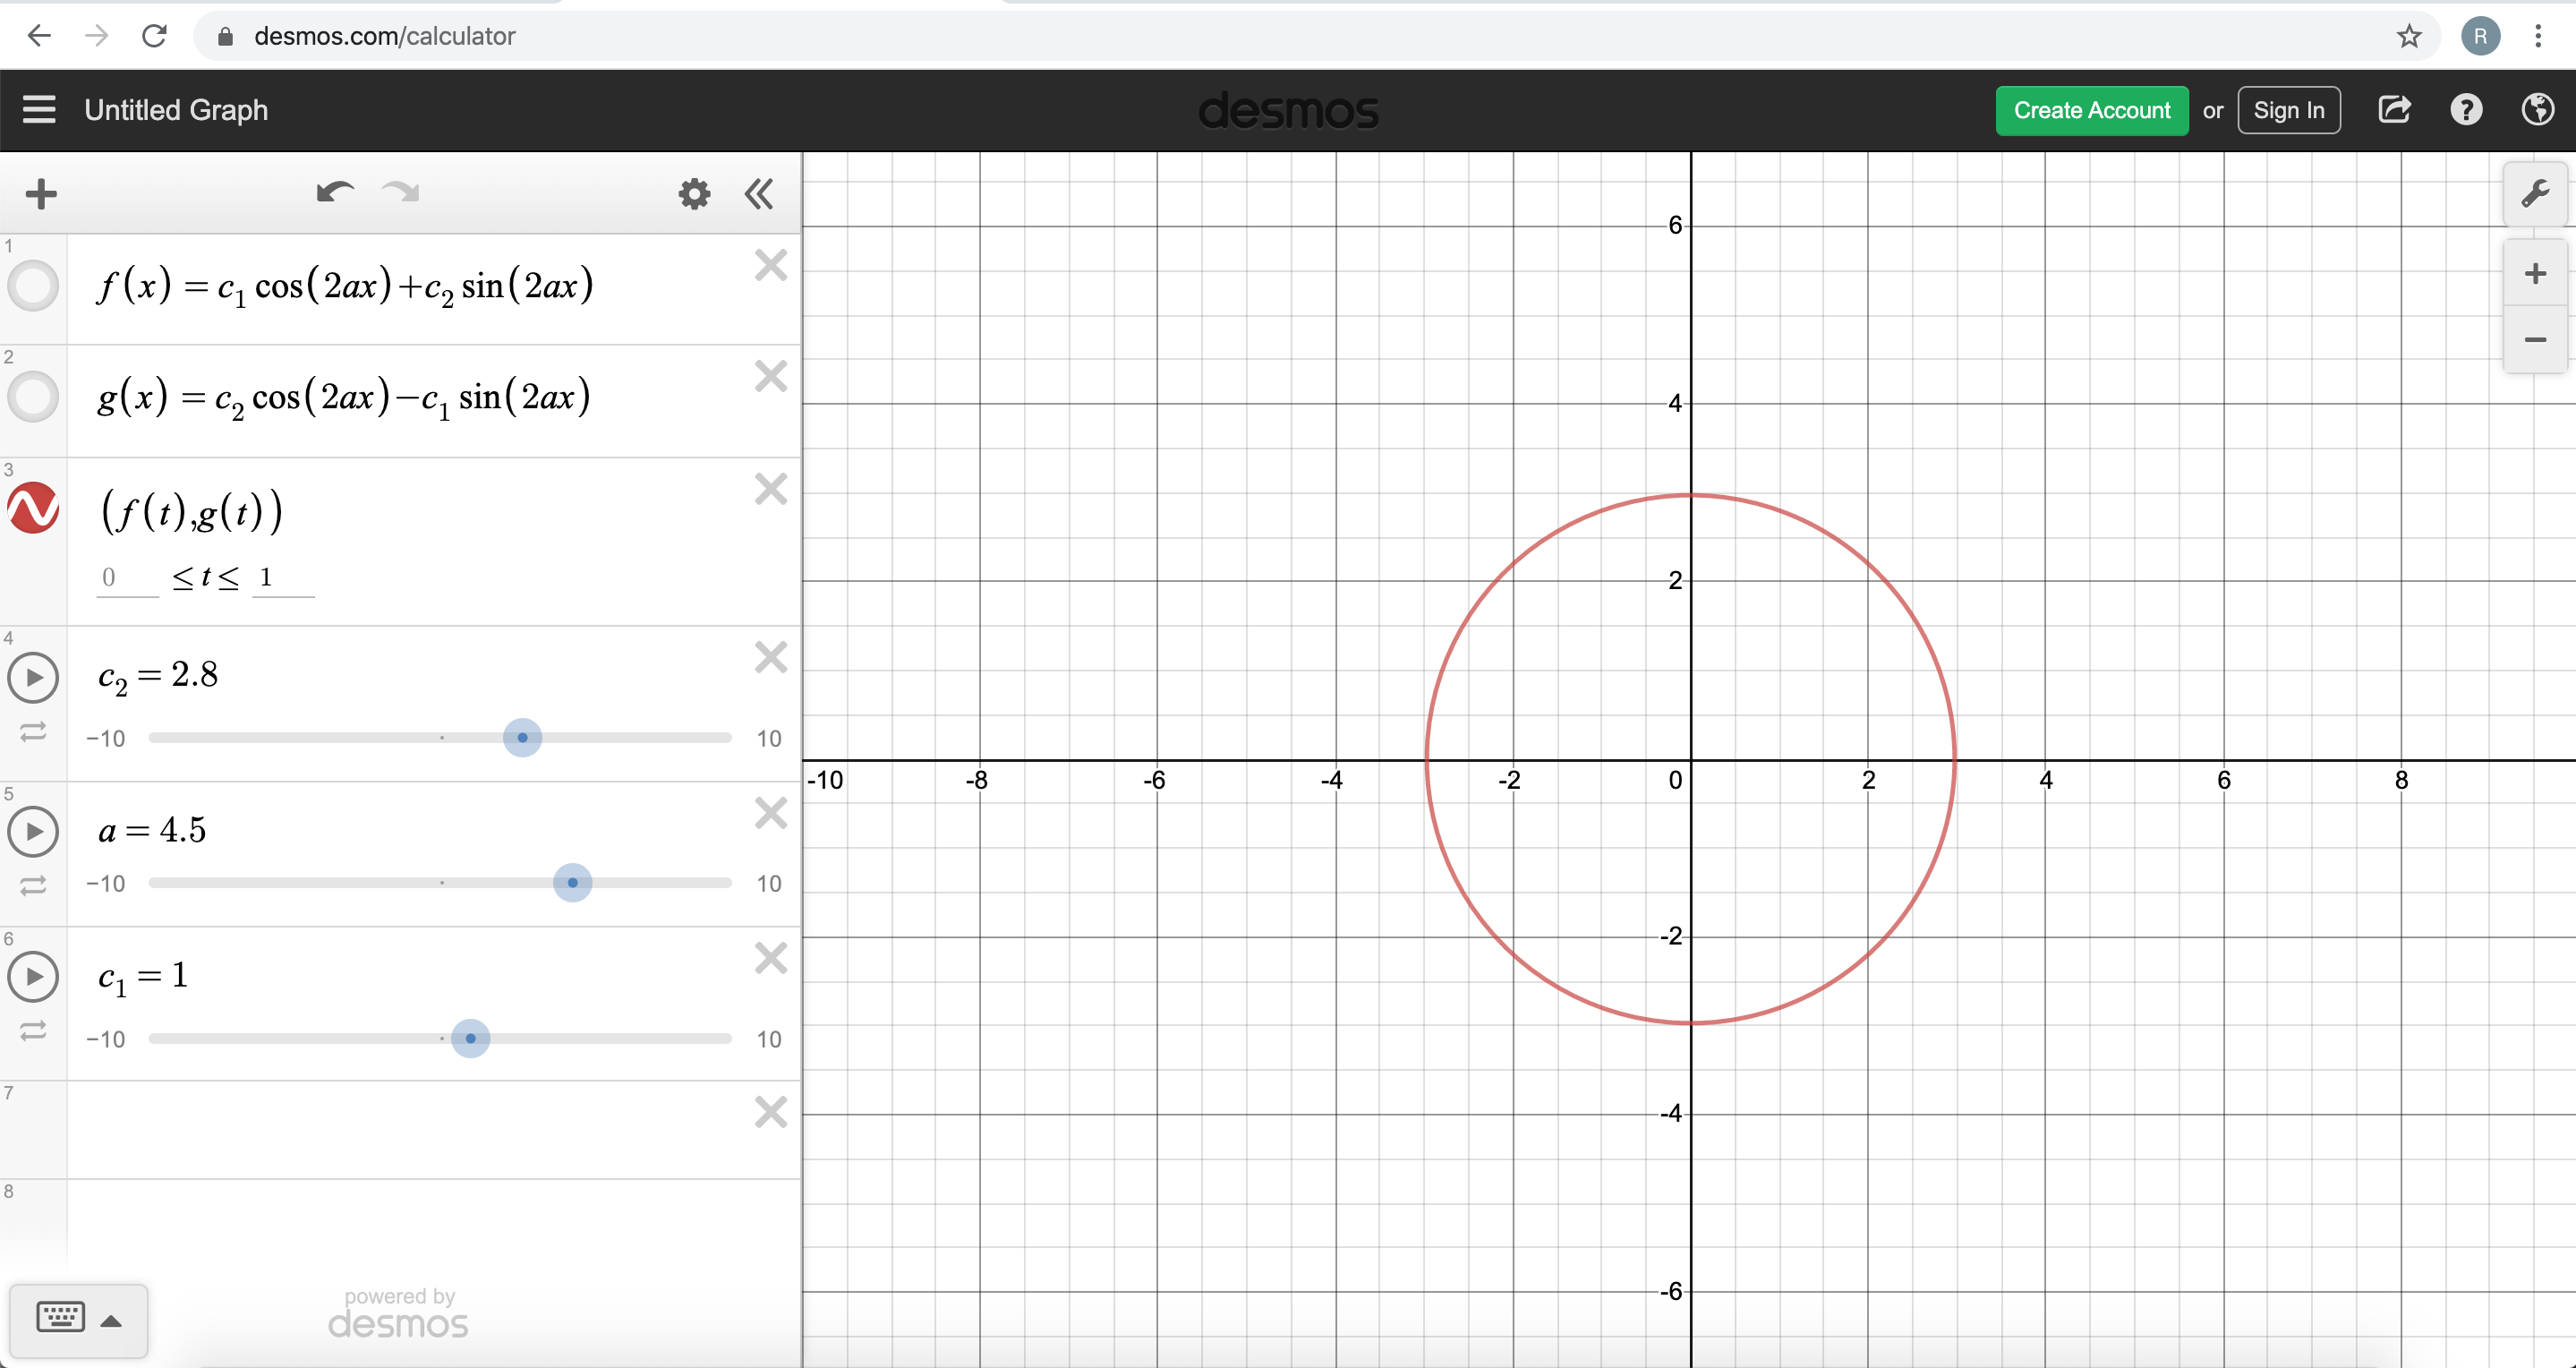
\includegraphics[width=\textwidth]{Figure1}
Changing $c_1$ and $c_2$ affects the size of the circle.
Changing $a$ only affects the paramaterization.

Now let's begin an analysis of the radius of the circle.
Notice that $z\bar z=(f+g)(f-gi)=f^2+g^2$, which is the radius of our circle. 
Since this is a constant with respect to time, we should expect $\frac{d}{dt}\left(z\bar z\right)=0$.
Let's check this assumption:
\begin{align*}
\frac{d}{dt}\left(z\bar z\right)&=\dot z\bar z+z\dot {\bar z}\\
&=(-2aiz)\bar z+z\overbar{(-2aiz)}\\
&=(-2aiz)\bar z+z\overbar{(-2ai)}\bar z\\
&=(-2aiz)\bar z+z(2ai)\bar z\\
&=0
\end{align*}
So if the radius of the circle never changes it is just equal to the initial value $z(0)\bar z(0)$.

\section{Assuming $\beta$ is real, a=d=0}

Let $\beta=b\in\mathbb R$.
Recall our ODE.
$$\dot{\begin{pmatrix}x\\y\end{pmatrix}}=A{\begin{pmatrix}x\\y\end{pmatrix}}, A=\begin{pmatrix}0&\beta\\-\beta&0\end{pmatrix}$$
Here we are going to take a different approach than what we did in section 4. As we saw when $\beta=0$ the matrix:
\begin{align*}
A = \begin{pmatrix}ai&0\\0&-ai\end{pmatrix}
\end{align*}
results in a situation where $z = constant$ since $\frac{d}{dt} z\bar{z} = 0$. For our current assumptions we have:
\begin{align*}
A = \begin{pmatrix}0&b\\-b&0\end{pmatrix}
\end{align*}
and it follows that we could diagonalize this matrix to get the same situation as the previous case where $b = 0$. To diagonalize the matrix above we need to find a matrix $T$ such that:
\begin{align*}
T\begin{pmatrix}0&b\\-b&0\end{pmatrix}T^{-1}
\end{align*}
is diagonal. Furthermore we need to modify the original system of equations we started with.
\begin{align*}
\dot{\begin{pmatrix}x\\y\end{pmatrix}}&=\begin{pmatrix}0&b\\-b&0\end{pmatrix}\begin{pmatrix}x\\y\end{pmatrix}\\
T\dot{\begin{pmatrix}x\\y\end{pmatrix}}&=T\begin{pmatrix}0&b\\-b&0\end{pmatrix}\begin{pmatrix}x\\y\end{pmatrix}\\
T\dot{\begin{pmatrix}x\\y\end{pmatrix}}&=T\begin{pmatrix}0&b\\-b&0\end{pmatrix}T^{-1}T\begin{pmatrix}x\\y\end{pmatrix}
\end{align*}
Now we have the original system in terms of the diagonal matrix that we want. To simplify, let: 
\begin{center}
$\begin{pmatrix}u\\v\end{pmatrix}=T\begin{pmatrix}x\\y\end{pmatrix}$
\end{center}
Then
\begin{center}
$u = T_{1,1}x + T_{1,2}y$\\
$v = T_{2,1}x + T_{2,2}y$
\end{center}
To find T we need to find the eigenvalues and their corresponding eigenvectors for the matrix:
\begin{align*}
A = \begin{pmatrix}0&b\\-b&0\end{pmatrix}
\end{align*}
Which are
\begin{center}
$\lambda_{1} = ib$, $v_{1} = \begin{pmatrix}1\\i\end{pmatrix}$\\
$\lambda_{2} = -ib$, $v_{2} = \begin{pmatrix}i\\1\end{pmatrix}$\\
\end{center}
Thus
\begin{align*}
T &= \begin{pmatrix}1&i\\i&1\end{pmatrix}\\
T^{-1} &= \begin{pmatrix}\frac{1}{2}&\frac{-i}{2}\\[6pt]\frac{-i}{2}&\frac{1}{2}\end{pmatrix}\\
\end{align*}
Plugging the values of T into the previous system involving $u$ and $v$ we get
\begin{center}
$u = 1x + iy$\\
$v = ix + 1y$
\end{center}
Now we want to consider $|vu^{-1}|$ similarly to when we considered $z=yx^{-1}$ which gives us
\begin{center}
$vu^{-1} = \mathLarge{\frac{ix + y}{x + iy}}$
\end{center}
We can write this in terms of $z$ with some manipulation as follows
\begin{center}
$vu^{-1} = \mathLarge{\frac{ix + y}{x + iy}}\cdot\mathLarge{\frac{x^{-1}}{x^{-1}}}=
\mathLarge{\frac{i + yx^{-1}}{1 + iyx^{-1}}} = \mathLarge{\frac{i + z}{1 + iz}}$
\end{center}
Therefore
\begin{center}
$|vu^{-1}| = \mathLarge{\frac{|i + z|}{|1 + iz|}} = c$
\end{center}
where $c \in \mathbb R$ is a constant. Letting $z=f + ig$ we get.
\begin{center}
$\mathLarge{\frac{|f + (1+g)i|}{|(1-g) + if|}} = c$
\end{center}
Now we can solve this for $f$ to get the shape of this equation.
\begin{align*}
\mathLarge{\frac{\sqrt{f^{2} + (1+g)^{2}}}{\sqrt{(1-g)^{2} + f^{2}}}} &= c\\
\mathLarge{\frac{f^{2} + (1+g)^{2}}{(1-g)^{2} + f^{2}}} &= c^{2}\\
f^{2} + (1+g)^{2} &= c^{2}((1-g)^{2} + f^{2})\\
f^{2} + (1+g)^{2} &= c^{2}(1-g)^{2} + c^{2}f^{2}\\
f^{2} + c^{2}f^{2} &= c^{2}(1-g)^{2} - (1+g)^{2}\\
f^{2}(1-c^{2}) &= c^{2}(1-g)^{2} - (1+g)^{2}\\
f &= \mathLarge{\sqrt{\frac{c^{2}(1-g)^{2} - (1+g)^{2}}{1-c^{2}}}}
\end{align*}
Using the same tool as in section 4 we can graph this equation as well to see its shape. Note that since $f$ represents the real part of $z$ while $g$ represents the imaginary part the axes are inverted.\\\\
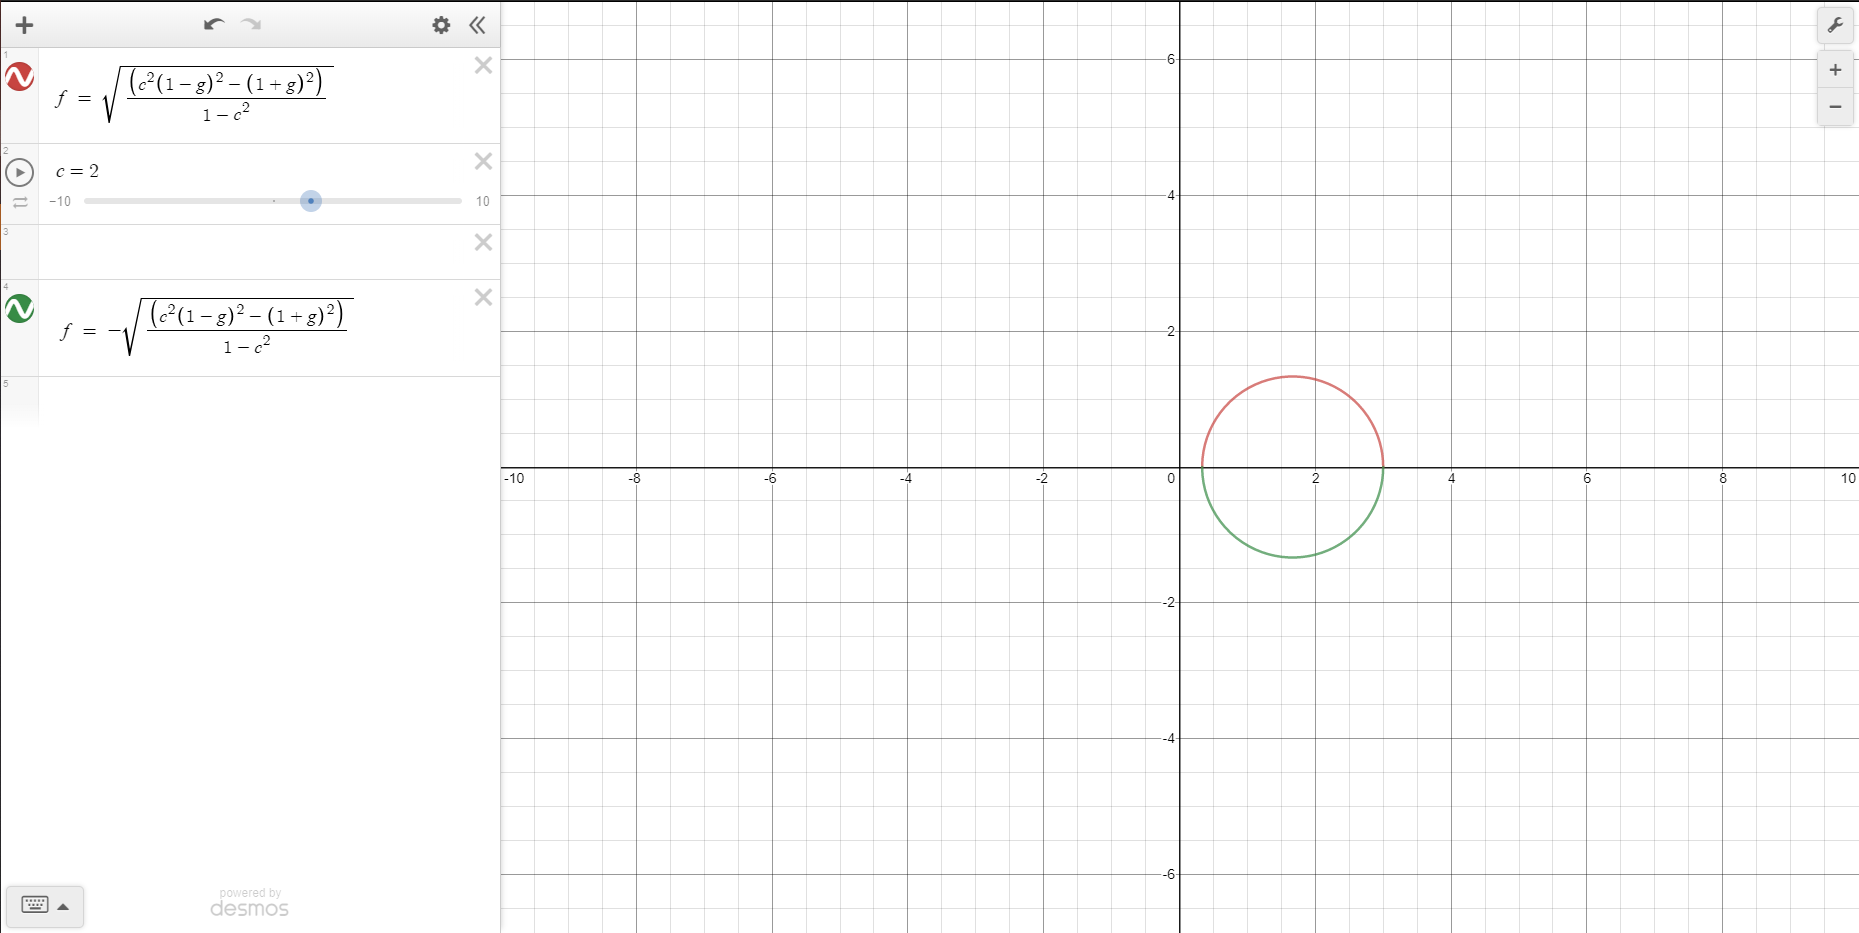
\includegraphics[width=\textwidth]{Figure3}\\
Here, $c$ controls both the center of the circle and the radius, where $c\neq1$



\section{Assuming $\beta$ is purely imaginary, a=d=0}
Let $\beta = bi$ where $b\in\mathbb{R}$ then our matrix look like:
\begin{center}
$A = \begin{pmatrix}0&bi\\bi&0\end{pmatrix}$
\end{center}
We can take the same approach here as described in section 5. The eigenvalues and eigenvectors of $A$ are:
\begin{center}
$\lambda_1=bi, v_1=\begin{pmatrix}1\\1\end{pmatrix}$
$\lambda_1=-bi, v_1=\begin{pmatrix}-1\\1\end{pmatrix}$
\end{center}
Thus the matrix $T$ we are looking for is:
\begin{center}
$T = \begin{pmatrix}1&-1\\1&1\end{pmatrix}$
\end{center}
Plugging the values of $T$ into the system with $u$ and $v$ gives us:
\begin{align*}
u = 1x+-1y &= x-y\\
v = 1x+1y &= x+y
\end{align*}
Then:
\begin{center}
$|vu^{-1}|= \mathLarge{\frac{x + y}{x - y}}\cdot\mathLarge{\frac{x^{-1}}{x^{-1}}}=
\mathLarge{\frac{1 + yx^{-1}}{1 - yx^{-1}}} = \mathLarge{\frac{1 + z}{1 - z}} = c$
\end{center}
For some $c\in\mathbb{R}$. Letting $z=f+gi$ for $f,g\in\mathbb{R}$, and solving for $g$ results in:
\begin{center}
$g = \mathLarge{\sqrt{\frac{c^{2}(1-f)^{2} - (1+f)^{2}}{1+c^{2}}}}$
\end{center}
The equation above results in a few possible shapes depending on the value of $c$.\\
If $c>1$ or $c<-1$:\\\\
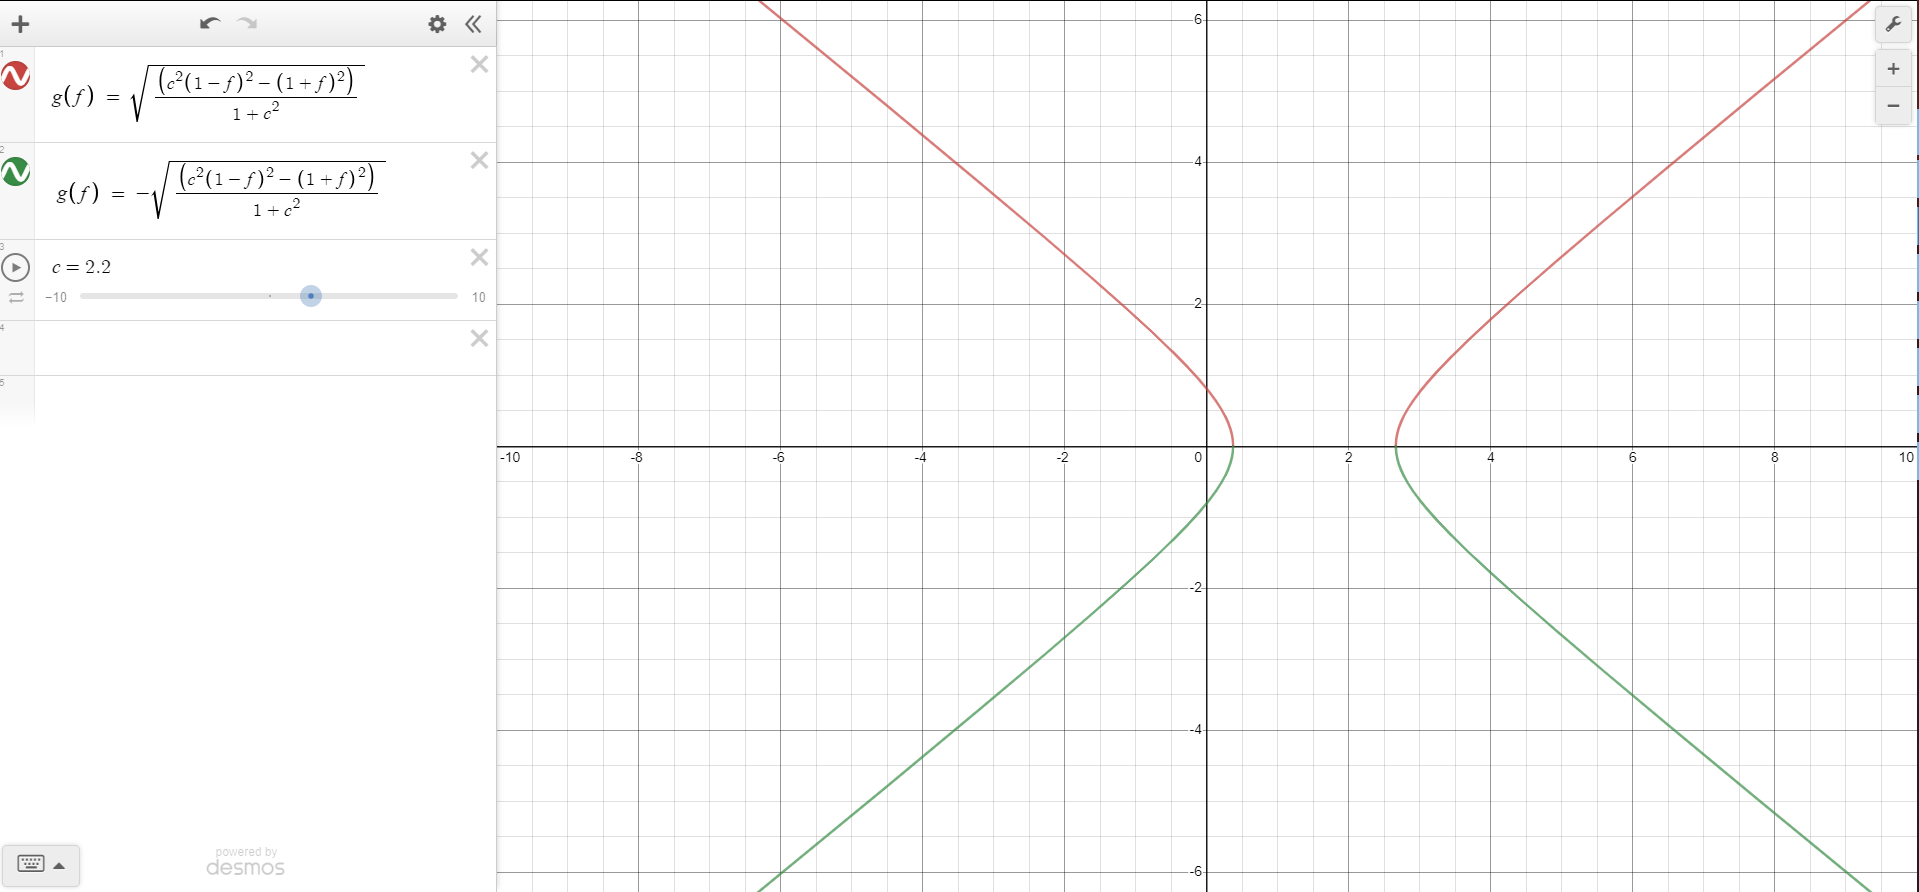
\includegraphics[width=\textwidth]{Figure4}\\
When $c>1$ or $c<-1$ we get a hyperbola whose center and focal points change as $c$ changes.\\\\
If $-1\leq c\leq1$:\\\\
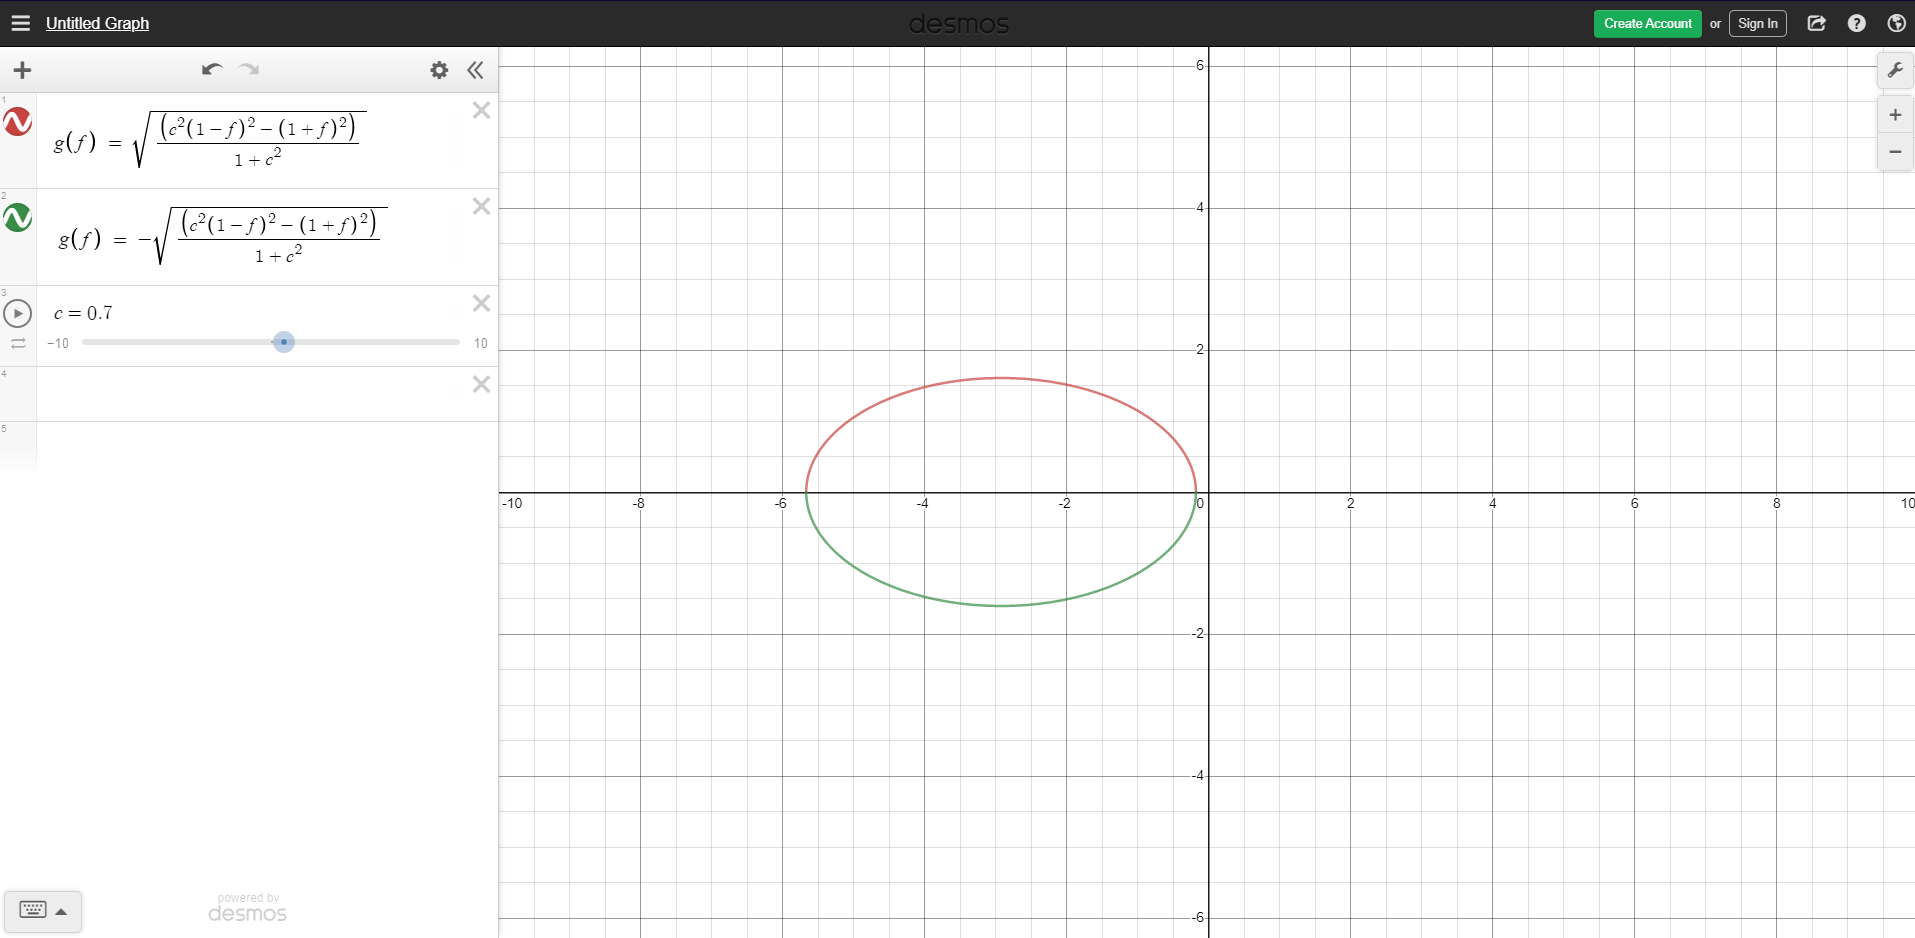
\includegraphics[width=\textwidth]{Figure5}\\
When $-1\leq c \leq 1$ we get an ellipse or circle whose center and focal points change as $c$ changes between this interval.











\end{document}